\documentclass[12pt]{article}
\usepackage{graphicx}

\begin{document}
\begin{titlepage}
\begin{center}

\includegraphics[scale=1]{diagrams/up.png}
\\
\begin{huge}
\textbf{2017 Class Project}
\textbf{NavUP}\\
\end{huge}
\hfill \break
\begin{huge}
\begin{center}
\textbf{Team Broadsword Team Navigation Module}
\end{center}
\end{huge}
\hfill \break
\hfill \break
\begin{small}
	Bondjobo, Jocelyn 	13232852 \\
	du Plooy, Andries	15226183 \\
	Brijlal, Yashvir		14387744 \\
	Jones, Keanan		13036892 \\	
	Nxumalo, Banele		12201911 \\
	van Schalkwyk, John	14307317 \\
\end{small}

\end{center}
\end{titlepage}

\newpage
\pagenumbering{arabic}
\thispagestyle{empty}
\tableofcontents
\clearpage


\section{Navigation Module}
\subsection{Scope}
Navigation employs a caching mechanism whereby commonly used routes are stored within a database in order to mitigate the cost of calculating popular routes multiple times.  Additionally, it acts as the Controller in the Model-View-Controller architecture with Access acting as the View and GIS being the model.  The precise nature of the scope of the Navigation module is shown in the diagram below.

\begin{figure}[h]
\centering
\includegraphics[scale=0.5]{diagrams/navUse.png}
\end{figure}
\begin{itemize}
\item Get Route: Routes need to be calculated, thus the GIS module is queried in order to get the route.

\item Cache Route: Routes are persisted to avoid recalculation, thus popular routes with similar user preferences will be readily available.

\item Set User Preferences: The user's prefernces are stored locally, in order for the correct path for each user to be calculated.
\end{itemize}
 

\subsection{Domain Model}
\begin{figure}
\centering
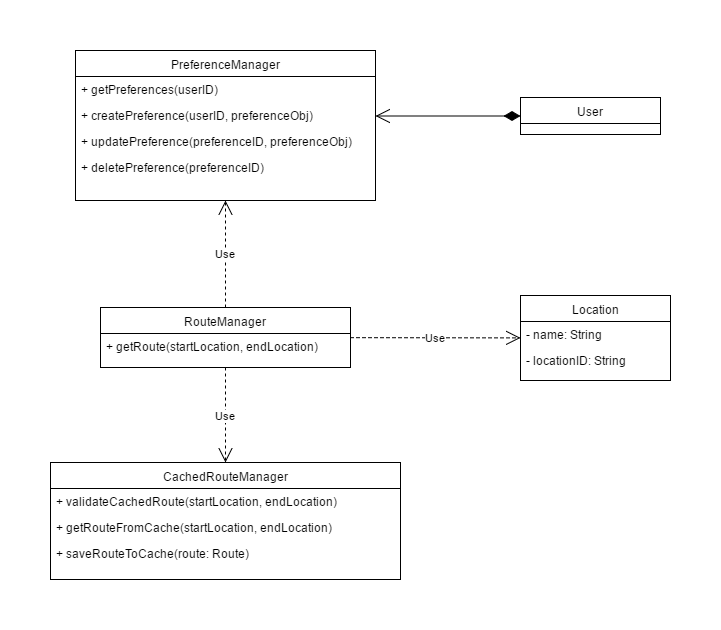
\includegraphics[scale=0.5]{diagrams/navigationDomainModel.png}
\end{figure}
The domain model encapsulates a simplified model of the core functionality provided within the navigation module. The route manager class handles route requests by receiving a start and end point and retrieving the route either from cache or, if not present in cache, retrieving it from the GIS module. 
The cached routes manager handles creating, saving and updating of cached routes through its various functions.
User preferences are required to retrieve filtered routes. The preference manager encapsulates creating retrieving updating and deleting of users preferences to be used by the route manager in retrieving filtered routes based on a users preferences.

\subsection{Service Contracts}
\begin{figure}[!htb]
\centering
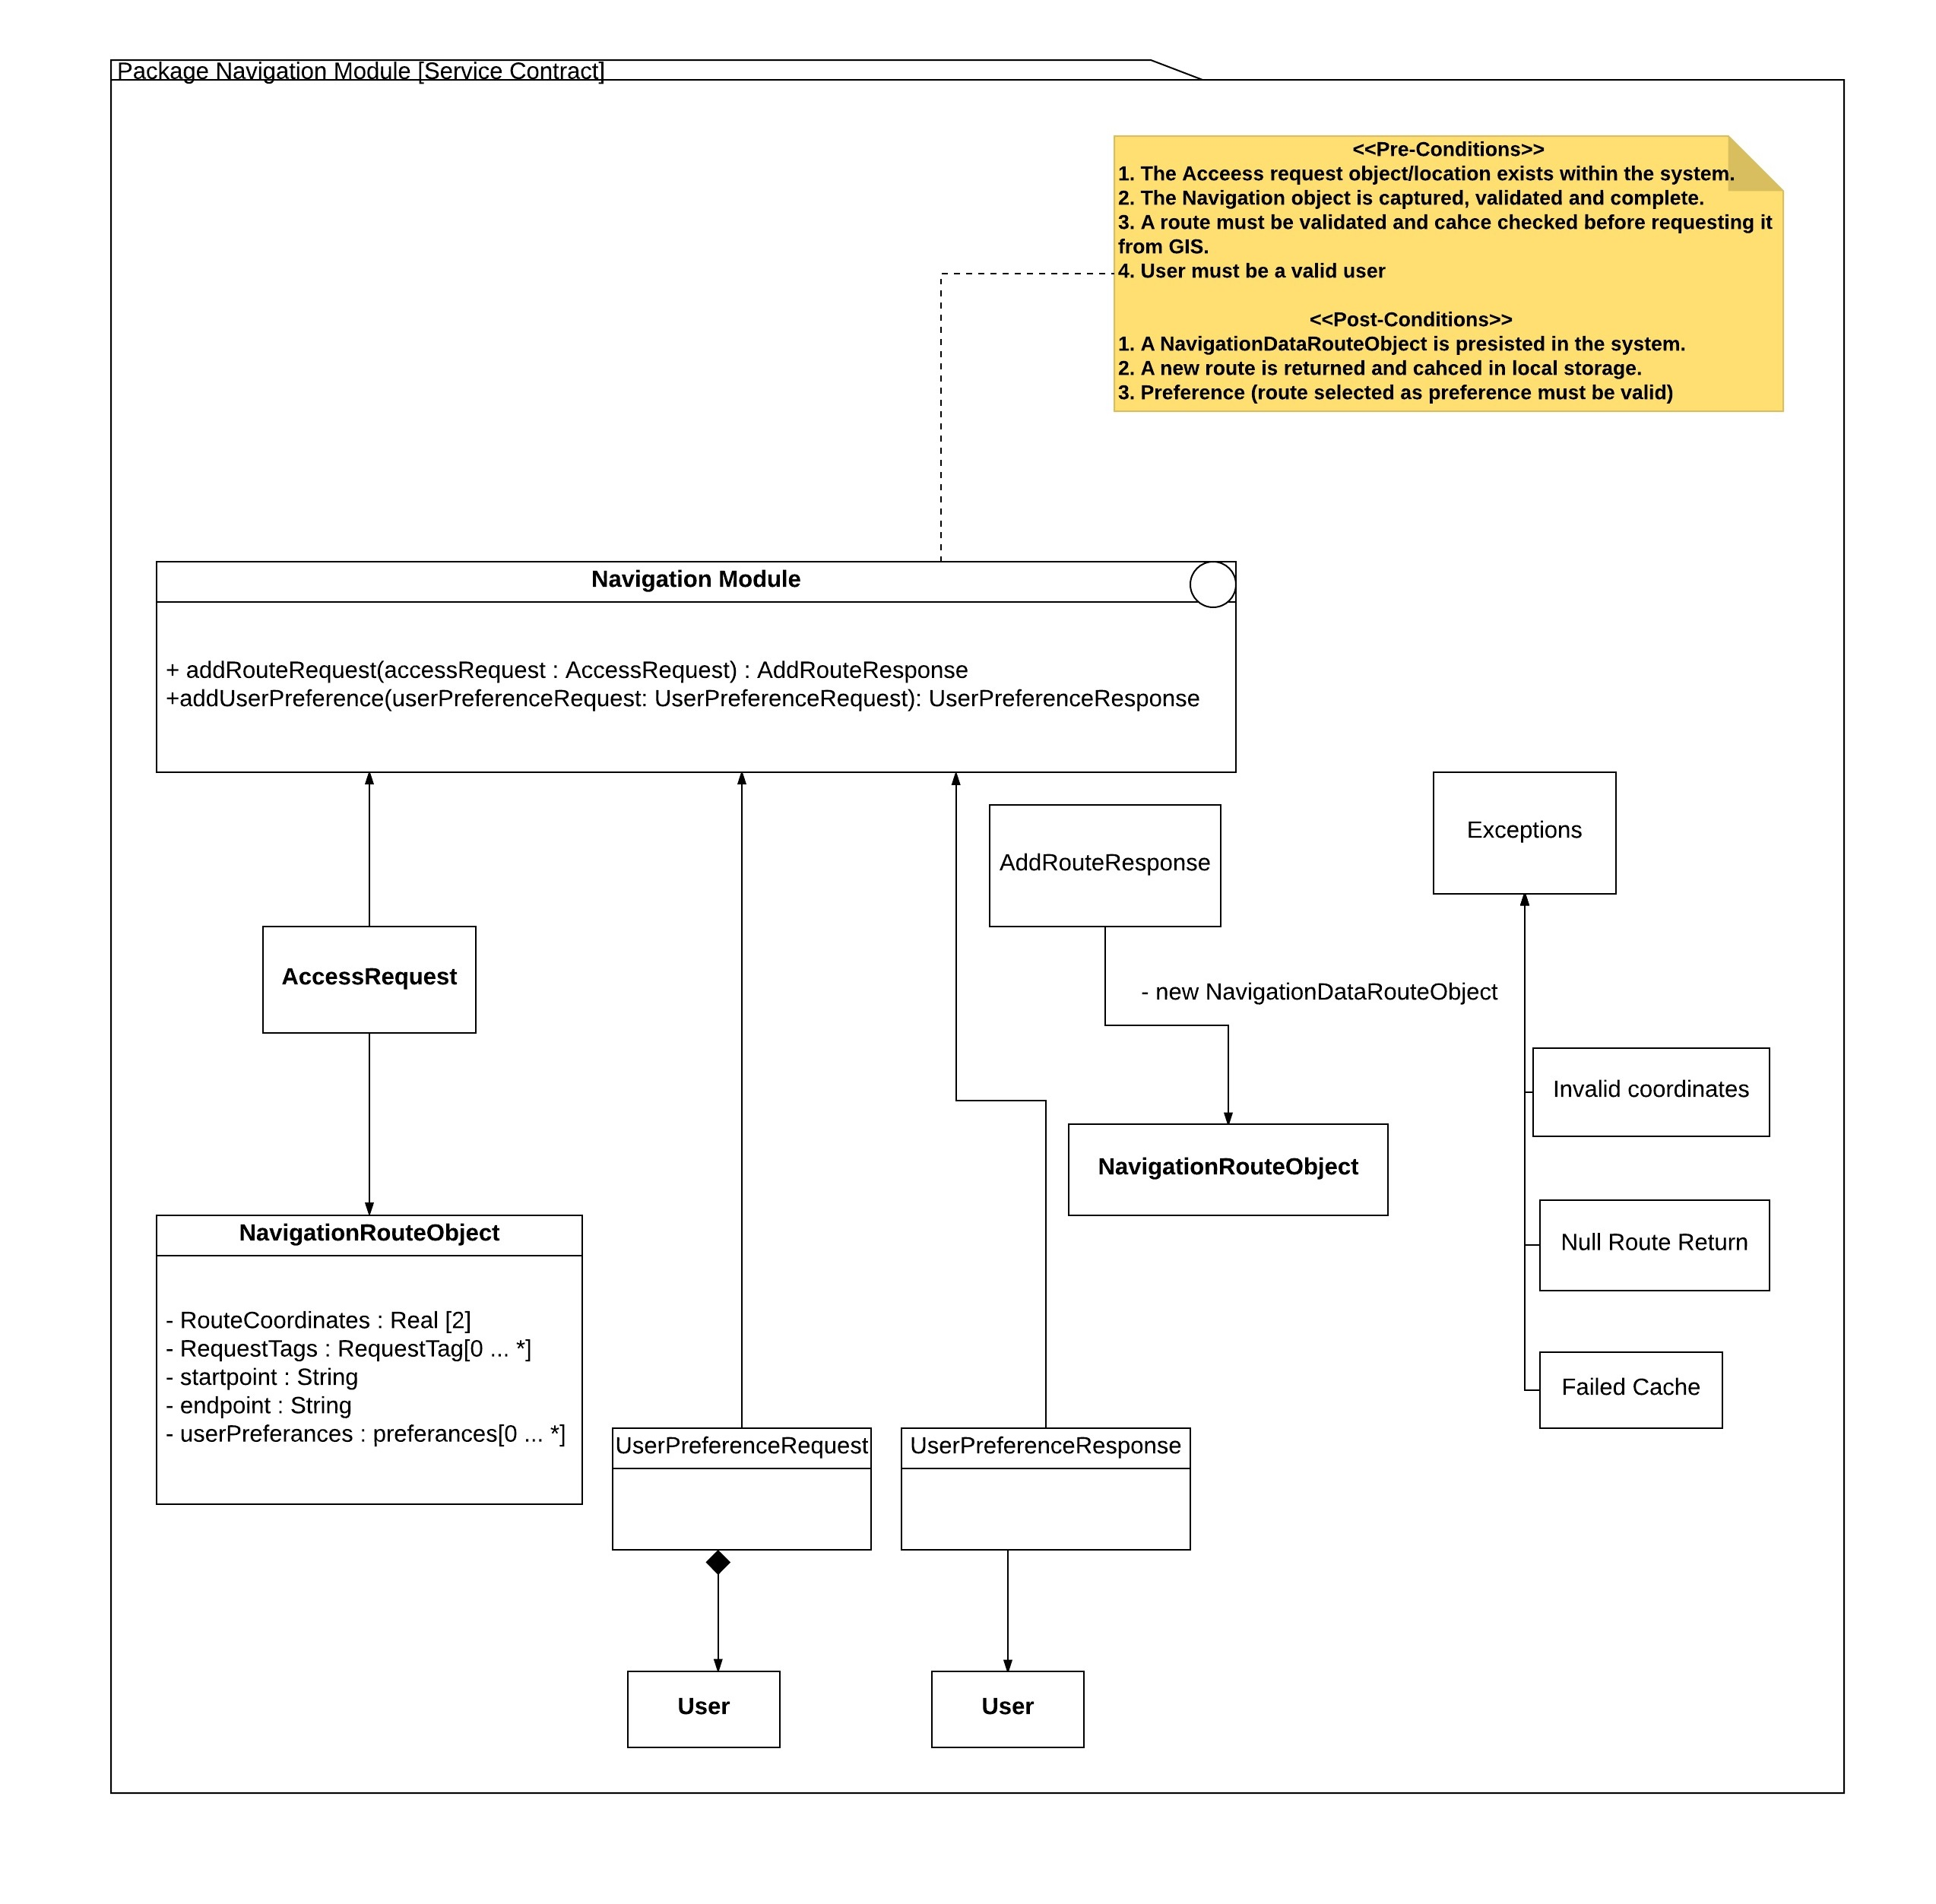
\includegraphics[scale=0.4]{diagrams/Service_Contract.jpeg}
\end{figure}
The reasons for which the service contract will fail can be due to a few actions occuring. 
\begin{itemize}

\item Firstly, When incorrect start and end locations are sent to the Navigation system, the system will not recognise it and will not return a route. Thus the correct desired start and endpoints must be received.


\item  A second occurance can be when the GIS module does not find a route, resulting in a null being returned. The null retuns must be handles as they will invalidate cached routes.
\end{itemize}

The only time GIS will be queries is the first time every route is requested. After that first request local cache will first be queried, thus reducing networking as well as request speed.


\subsection{Technology}
\subsubsection{MEAN STACK}  
	MEAN stack is the best solution for building application using javascript and since we are implementing the MVC architectural pattern for the navUP system , MEAN stack is the best way to deploy the current architectural pattern . It includes mongo , express , angular and nodejs which allows us to built fast and maintable applications.
\subsubsection{MongoDB}	
MongoDB is a document-oriented database that provides high perfomace,availability and scalability. It works on the concepts of collection and documents. For the NavUP application , we used mongoDB to store data such as startpoint,endpoint or user preferences.
\subsubsection{Express}
Express is fast and flexible framework for nodejs . 
\subsubsection{Nodejs}	
 Nodejs is JavaScript run-time environment for executing JavaScript code server-side. It is used for easily building fast and scalable applications. All the APIs of nodejs library are asynchronous means a Node.js based server never waits for an API to return data. 
 \subsubsection{Mongoose}
 This will be our Object Relational Mapping tool which will allow us to intuitively
 persist objects straight into the database. Mongoose allows us to have access to the MongoDB commands for CRUD  easily
 \subsubsection{NSQ} 
NSQ is a library used for communications between different modules like access ,gis and navigation modules. 

\end{document}